\chapter{Sesnando}
\label{ch:4}

This section introduces the SESNANDO project by describing the software operability and its core functionalities.

\section{Requirement analysis}
\label{sec:requirement_analysis}

The activity of identifying software functionalities and behavior is described as \textit{Requirements Engineering}. Before proceeding to the presentation of the SESNANDO architecture those will be identified in a simple manner.

\begin{itemize}
\item The application must be able to recognize a requirement identified by its keyword REQUIREMENT.
\item The application must be able to identify \textit{Given}, \textit{When} and \textit{Then} predicates.
\item The application must extract Logical Expressions between \textit{AND} and \textit{OR} boolean operators.
\item The application must identify Logical Expressions using the operators: \textit{Equal than}, \textit{Lower Than}, \textit{Lower Than or Equal}, \textit{Greater Than} and \textit{Greater Than or Equal}.
\item The application must be able to identify Requirement Signals (Logical Signals) within a Logical Expression.
\item The application must be able to identify an Operand within a Logical Expression.
\item The application must be able to identify a Logical Expression Quantifier, i.e., the system components to which the expression shall be evaluated, e.g., a train axle.
\item The application must be able to compile the requirement into a Parse tree.
\item The application must be able to access the Parse Tree and generate a set of test cases from the interpreted requirements.
\item The application must be able to generate a standard output file (CSV) containing a set of test cases.
\item The application must be able to generate a test script to be used on the testing environment.
\end{itemize}



\section{Software Architecture}
\label{sec:software_architecture}

Sesnando is divided into multiple modules that communicate with each other. Next those modules will be presented as well as their main roles within sesnando. \\

\begin{figure}[h]
    \centering
    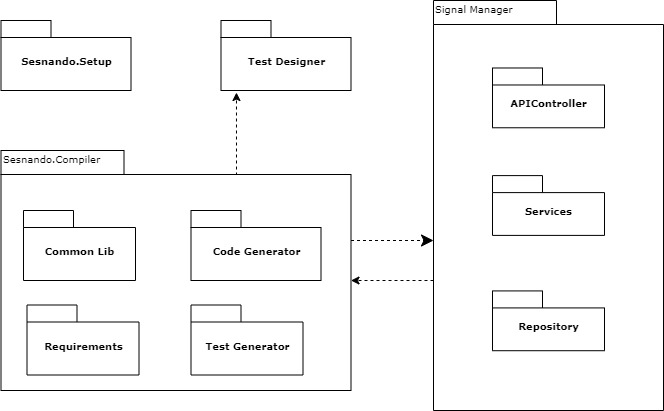
\includegraphics[scale=0.625]{images/sesnando_modules.jpg}
    \caption{Main application modules}
\end{figure}
\label{fig:sesnando_modules}

\begin{itemize}

\item Sesnando.Setup - Is responsible to verify and install all the Application dependencies on the operating system.

\item Sesnando.Compiler - Is the entry point of this Application and will call all the relevant modules as needed.

\item Requirement Module - This module will be called in the beginning of the program execution. It will read the input requirements and will then parse its contents using an Abstract Syntax Tree, i.e. it contains a predefined grammar that will be used to compile the requirement into a set of Objects. Those will be detailed further within this document.

\item Test Generator - Once the object tree is successfully constructed, this module will be notified to extract the required data from it in order to start to define the first tests, the Object tree will be then mutated to generate new test cases.

\item Common Lib - Where the actual Abstract Syntax Tree objects will be stored, accessible to the whole application suite.

\item Signal Manager - The conversion of the Input requirements into Object trees is not direct and trivial. Signal Manager is a detachable service that contains a database with the purpose to provide low-level technical context to the requirements, i.e., the requirement describe the functionalities on a high-level of abstraction which will be then mapped to a set of software signals ready to be used on the test environment. This is how the application can generate accurately software tests.

\item Code Generator - This module receives the standard output from the test generator and will then generate proper test artifacts compatible with the end test environment, e.g. test scripts.

\item Test Designer - Test designer is a detachable Graphical User Interface (GUI) module with the main purpose of displaying the generated test cases to the User. From this tool, the user is able to review, edit and export these test cases into a permanent file.
\end{itemize}
